% Chapter 1

\chapter{Introduction} % Main chapter title

\label{chap:intro} % For referencing the chapter elsewhere, use \ref{Chapter1} 

%----------------------------------------------------------------------------------------

% Define some commands to keep the formatting separated from the content 
\newcommand{\keyword}[1]{\textbf{#1}}
\newcommand{\tabhead}[1]{\textbf{#1}}
\newcommand{\code}[1]{\texttt{#1}}
\newcommand{\file}[1]{\texttt{\bfseries#1}}
\newcommand{\option}[1]{\texttt{\itshape#1}}

%----------------------------------------------------------------------------------------
In the recent past, significant progress has been made in neuroscience and artificial intelligence (AI). With the inception of computers in the early nineteenth century, progress in AI was inextricably intertwined with neuroscience and psychology, and many of the early pioneers straddled both fields, with collaborations between these disciplines proving highly productive \citep{turing1950computing, hinton1986distributed, mcculloch1943logical, hebb1949organization, churchland1988perspectives}. Nevertheless, progress in recent times has seen interactions and collaborations becoming less commonplace, as both fields have evolved massively in complexity, and disciplinary boundaries have solidified. 

The development of AI began with the premise that creating human like general purpose artificial intelligence (or ‘‘Turing-powerful’’ intelligent systems) is an intimidating task, due to the massive search space of sparsely populated solutions. This underscored the utility of examining the principles of the human brain which is the only existing proof that such an intelligence is even possible. As described by \citet{hassabis2017neuroscience}, the benefits of developing AI by close scrutinisation of biological intelligence are two-fold. First, neuroscience provides a rich source of inspiration for new algorithms and architectures, independent of and complementary to the mathematical and logic-based methods, and ideas that have largely dominated traditional approaches to AI. For example, where a new facet of biological computation found to be critical to supporting a cognitive function, then it has been considered as an excellent candidate for incorporation into artificial systems. Second, neuroscience can provide validation of artificial intelligence techniques that already exist. If a known algorithm is subsequently found to be implemented in the brain, then that is strong support for its plausibility as an integral component of an overall general intelligence system.
\section{Rationale and Motivation}

It is without a doubt that in the era of `smart' everything, availability and utility of massive volumes of digital data plays a substantial role. Historically, data was used as a part of business and gathered to serve specific needs. For example, retailers recorded sales for accounting, manufacturers recorded raw materials for quality management and the number of mouse clicks on advertising banners was collected for calculating advertisement revenue. But as the demand for big data analytics emerged, data no longer served only its initial purpose. Organisations were able to access huge amounts of data and possess a valuable asset that when combined with the ability to analyse it, has given rise to a whole new industry.

This thesis began its journey in the middle of a technological revolution in the year 2014 when the industry was booming with the following technological revolutions:
\begin{itemize}
	\item Big data: The total volume of digital data has grown into Zetabytes and is projected to be reaching $180$ Zetabytes by the year 2025. This enormous growth in digital data has brought on an era of "Big data". Big data is a term applied to data sets whose size or type is beyond the capabilities of traditional relational databases to capture, manage, and process the data with low-latency. Also, it has one or more of the following characteristics: high volume, high velocity, or high variety. Big data traditionally originates from Internet of Things (IoT) enabled sensors, devices, video/audio, networks, log files, transactional applications, and social media - much of it generated in real time and on a very large scale.
	
	\item Deep learning: Deep learning is a specialised stream of AI which has come into prominence in the past decade. Deep learning is considered to be an extension of machine learning, which consists of a set of technologies around neural networks that empowers computers to learn, evolve and improve upon their own learning by reiterating and consistently updating the data bank through recursive experiments and human intervention. Deep learning has already revolutionised AI and pushed the boundaries of intelligent systems through technologies such as autonomous cars, fully automated language translation and speech transcription systems. 
	
	\item High performance computing (HPC): Experts have described deep learning as analogous to a rocketship that needs a really big engine (a model) and a lot of fuel (the data) in order to go anywhere interesting. A big model that learns from big data, of course, requires large scale computational capabilities, or, in other words, high performance computing for it to be efficient and effective. The need for HPC has also meant a massive progress in the form of cloud computing and infrastructure as a service providing capability to scale infrastructure requirements (computation, storage, network speed) on a demand basis.  
	
\end{itemize}

The state-of-the-art of AI is composed of big data, big models and big infrastructure where solutions are traditionally developed by stacking up resources in the form of multiple instances of computers (physical and/or logical). The main motivation and/or question that drives the present research in this domain is the following: "Is stacking up computers an ideal solution for the future direction of AI?" This question led to the revisiting of the field of neuroscience seeking inspiration from biological intelligence for efficient and accurate computing. 

An important distinction of the human brain from AI is its ability to operate at full capacity using orders of magnitude lower power. This is a rather subtle hint that the human brain does not scale by stacking up computational units. Rather, the efficiency is due to the ability of the human brain to represent sensory information as electrical impulses. The idea of information representation as electrical impulses is at the base of this thesis. The present work concentrates on developing algorithms for pattern recognition, not by stacking layers of computational units and infrastructure, rather by developing algorithms for representing, processing and recognising patterns in big data, especially time-series data, efficiently and accurately.     


\section{Aims of this Thesis and Research Questions}
\label{sec:research_ques}
On the basis of the rationale and motivations discussed previously, this work constrains its focus on the development of neuromorphic computational models for recognising patterns using multi-modal time-series data.

\begin{enumerate}
	\item Neuromorphic models: This thesis concentrates on developing neuro-biology inspired computational models known as spiking neural networks for recognising patterns in data. The most important characteristic ensuring neuromorphic behaviour is the ability to represent, transform and process spike-time data. 
	\item  Multi-modal time-series data: As it has been briefly described earlier, the concept of big data is characterised not only by volume and velocity, but also very importantly, by variety. The data sources in the era of IoT are diverse, leading to multi-modal data with a variety of spatio-temporal properties. The aim is to develop technologies that has the capacities to deal with such multi-modal data sources.
	\item Time-series, especially brain data: The studies in this thesis are also limited to experiments performed on time-series data, especially, non-invasive brain data, such as functional Magnetic Resonance Imaging (fMRI), Electroencephalography (EEG), and Diffusion Tensor Imaging (DTI). The brain activity data is particularly useful as data sources of multi-modal nature with prominent impact on healthcare for several brain related diseases. This will be discussed in detail later.   
\end{enumerate} 
Keeping the above mentioned constraints in mind, this research aims to answer the following more in-depth research questions:

\begin{enumerate}
	\item \textbf{Research question 1}: How to design architectures of spiking neural networks that are capable of digesting and processing large volumes of spatio-temporal data? This research question focuses on software design principles, including the data structure design, modularity and scalability aspects of spiking neural network architectures.
	\item \textbf{Research question 2}: How to perform neural encoding on real-world data to represent information as timings of spikes? This research question can be observed in the light of information theory and theories of lossy data compression. 
	\item \textbf{Research question 3}: How to integrate spatial, temporal and orientation information present in multi-modal brain data using spiking neural network architecture?  
\end{enumerate} 

\section{Thesis Structure, Navigation and List of Peer-reviewed Publications}
\begin{sidewaysfigure}
\centering
	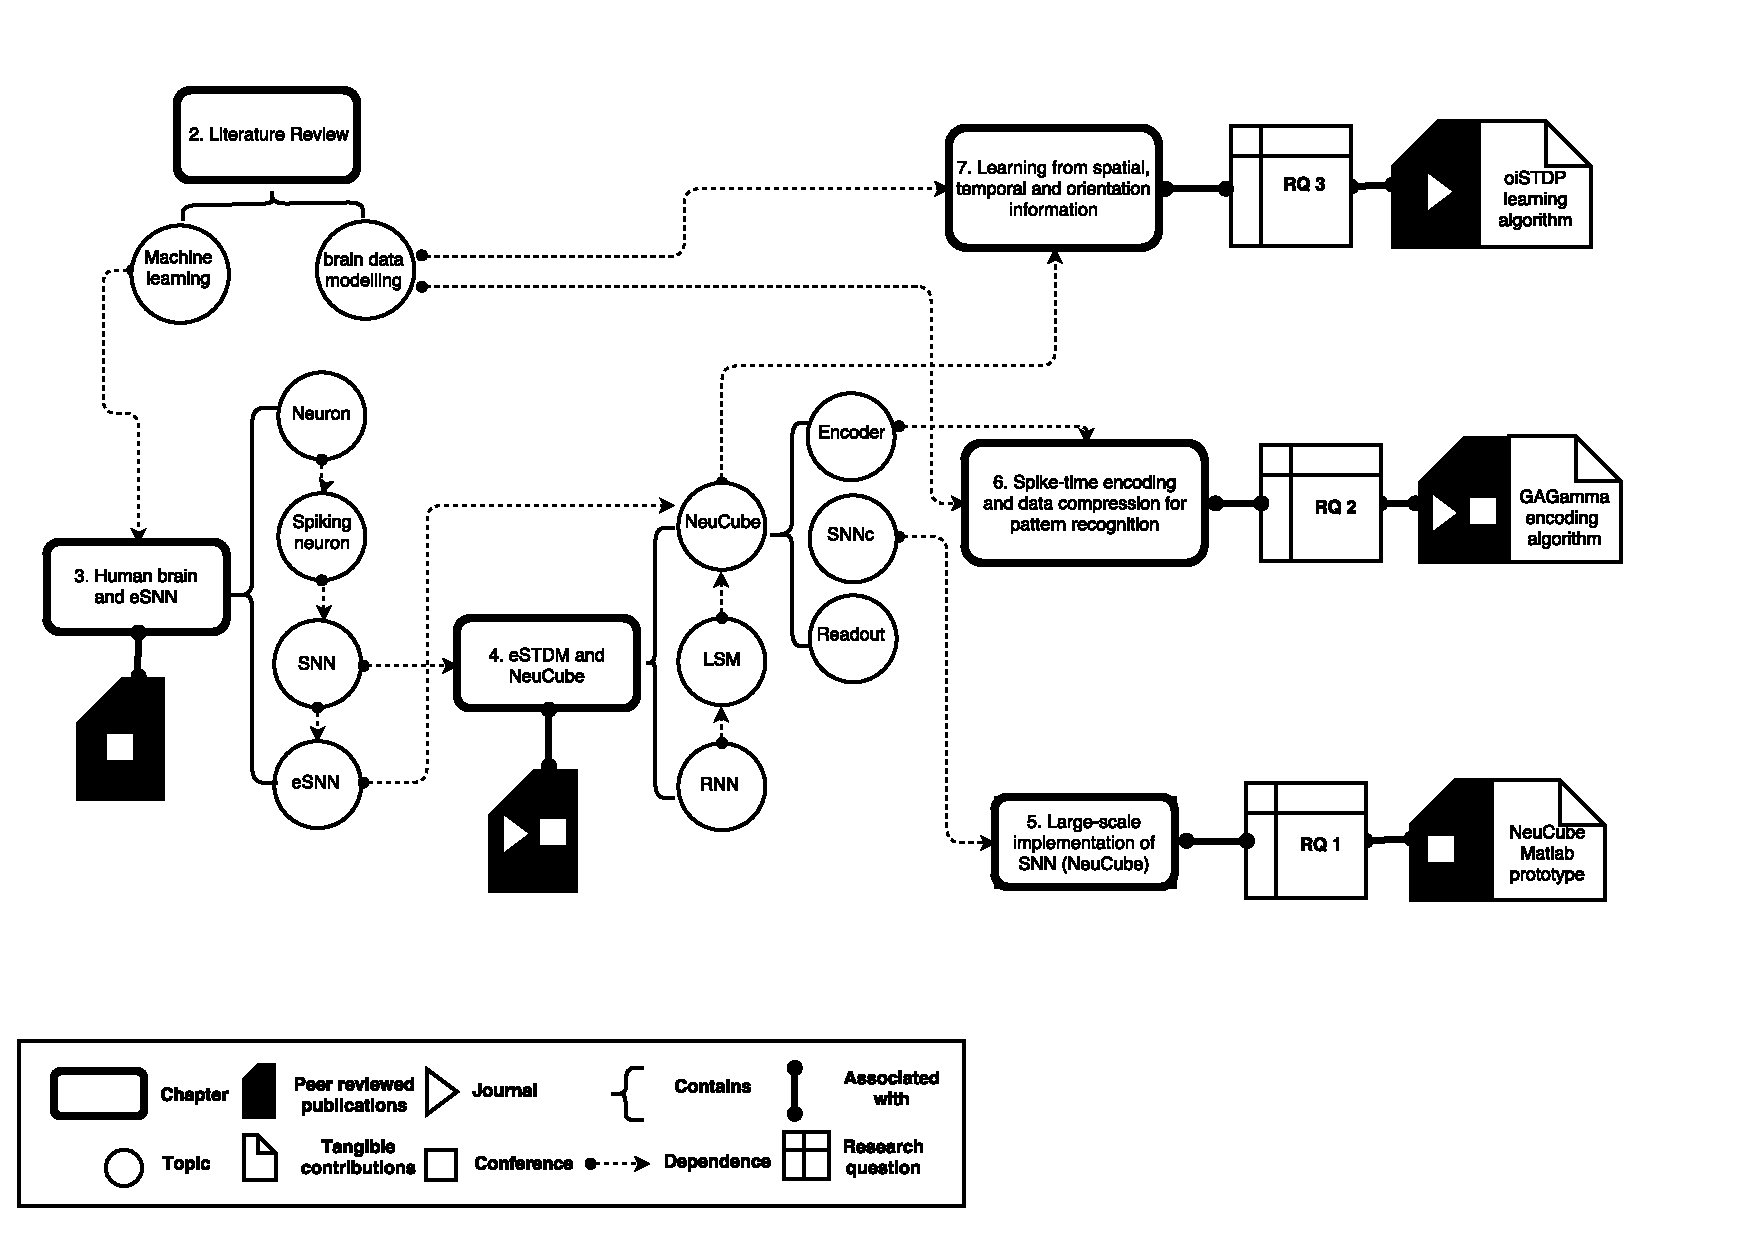
\includegraphics[scale=0.8]{fig/intro/Navigation.pdf}
	\caption{Bird's eye view of thesis components and their inter-dependence.}
	\label{fig:birds_eye}
\end{sidewaysfigure}

This thesis is presented in eight Chapters. \figurename \ref{fig:birds_eye} depicts a self-explanatory bird's eye view of the relationships between the different components of interest of this thesis. It is highly recommended to review this figure before proceeding further. The components are categorised as Chapters, topics, research questions, tangible outcomes (software implementations or algorithms) and publications (journals, conferences or book chapters). There are three categories of relationships (arrows in the diagram) drawn in the figure: (1) Contains: These are one-to-many relationships. A relationship of this kind can be observed between a chapter and multiple topics. (2) Dependence: These are directed one-to-one relationships. The one-to-one directed relationships are drawn between chapters and/or topics. Following the dependence graph, the reader can navigate through the prerequisites and/or flow of topics. (3) Associated with: These are undirected one-to-one relationships associating a pair of components (such as a Chapter and a research question, or a Chapter and a publication). An example of a possible navigation through the diagram is as follows: To read Chapter 7 for example (which is associated with research question 3 and resulted in one journal publication and a tangible outcome in the form of oiSTDP learning algorithm), a reader is recommended to read Chapter 2, especially the topics on brain data modelling and Chapter 4, especially the topics related to NeuCube (which also has certain prerequisites).

This thesis generally follows a linear and continuous flow. This means that efforts have been made throughout the thesis to cross-reference across chapters and sections in order to minimise repetitions. Chapter \ref{chap:large_snn}, \ref{chap:encoding} and \ref{chap:multimodal} are presented as the main contributions of this thesis and directly relates to the research questions discussed in section \ref{sec:research_ques}. Chapters \ref{chap:snn} and \ref{chap:neucube} on the other hand forms the basis on which the main chapters are written and many of the concepts are introduced in these chapters and reused thereafter in the main contributions. The following table lists the contributions that have been made in the form of peer reviewed publications through the work of this thesis. 
 
\begin{table}
		\centering
		\caption{List of peer-reviewed publications}
		\label{tab:publications}
	\begin{tabular}{@{}p{2cm}p{12cm}p{1cm}@{}}
			\toprule\toprule
			Type & Publication & Year \\ \midrule
			
			Journal & \textbf{Sengupta, N.}, McNabb, C. B., Kasabov, N. \& Russell, B. (2018), integrating space, time and orientation in spiking Neural Networks: A case study on multi-modal brain data modelling, IEEE Transactions on Neural Networks and Learning System. DOI: https://doi.org/10.1109/TNNLS.2018.2796023. & 2018 \\ \midrule
			
			Journal & \textbf{Sengupta, N.}, \& Kasabov, N. (2017). Spike-time encoding as a data compression technique for pattern recognition of temporal data. Information Sciences,  406, 133-145. & 2017 \\ \midrule
			
			Journal & Kasabov, N., Scott, N. M., Tu, E., Marks, S., \textbf{Sengupta, N.}, Capecci, E., ... \& Espinosa-Ramos, J. I. (2016). Evolving spatio-temporal data machines based on the NeuCube neuromorphic framework: design methodology and selected applications. Neural Networks, 78, 1-14. & 2016 \\ \midrule

			Conference & \textbf{Sengupta, N.}, Scott, N., \& Kasabov, N. (2015). Framework for knowledge driven optimisation based data encoding for brain data modelling using spiking neural network architecture. In Proceedings of the Fifth International Conference on Fuzzy and Neuro Computing (FANCCO-2015) (pp. 109-118). Springer, Cham. \\ \midrule
			
			Conference & Abbott, A., \textbf{Sengupta, N.} \& Kasabov, N. (2016). Which method to use for optimal structure and function representation of large spiking neural networks: A case study on the Neucube architecture. In 2016 international joint conference on neural networks(ijcnn)(pp. 1367-1372). IEEE & 2016 \\ \midrule
			
			Conference & Kasabov, N., \textbf{Sengupta, N.}, \& Scott, N. (2016, September). From von neumann, John Atanasoff and ABC to Neuromorphic computation and the NeuCube spatio-temporal data machine. In IEEE 8th International Conference on Intelligent Systems (IS), 2016  (pp. 15-21). IEEE. & 2016 \\ \midrule
			
			Conference & Arya, A. S., Ravi, V., Tejasviram, V., \textbf{Sengupta, N.}, and Kasabov, N. (2018, January) Cyber fraud detection using evolving spiking neural network, in IEEE International conference on industrial and information systems (ICIIS), 2016 (pp. 263-268). IEEE. & \multicolumn{1}{c}{2016} \\ \midrule
			
			Chapter & \textbf{Sengupta, N.}, Ramos, J.I.E., Tu, E., Marks, S., Scott, N.,... \& Abbott, A. (2018). From von Neumann architecture and Atanasoffs ABC to Neuromorphic Computation and Kasabov’s NeuCube: Principles and Implementations, Learning Sytems: From Theory to Practice. Springer. & 2018 \\ \bottomrule \bottomrule
	\end{tabular}
\end{table}












